\documentclass{article}

\usepackage{graphicx}
\usepackage{hyperref}
\usepackage{placeins}
\usepackage{subcaption}

\begin{document}

Machine Learning 2, exercise 1 by Constantin Pape, Marcus Theisen and Johann Klaehn
 
\section{Exercise and data}

In this exercise we compare different optimization methods for the problem of logistic regression.
The methods are tested on the digits dataset of sklearn.
We start by implementing vectorized versions of the sigmoid function and the gradient.
We further implement a function for prediction and a function to evaluate the error.

\section{Optimization methods}

For the optimization, we implement different methods:
First the gradient descent, then stochastich gradient descent and some variants of it.
As non-gradient based techniques, we use dual coordinate ascent and weighted least squares.

\section{Grid Search}

All gradient based methods depend on different parameters: The initial learning rate $\tau_0$, the learning update paramter $\gamma$ and for some methods an additional parameter $\mu$.
For the non-gradient based methods no parameters have to be optimized.
We perform a grid-search to find the best parameter (see \ref{tab1} for values).

\begin{table}[h]
	\centering
	\begin{tabular}{l c c c}
		$\tau_0$	&	0.001	& 0.01	& 0.1	\\
		$\mu$		&	0.1	& 0.2	& 0.5	\\
	 	$\gamma$ 	& 	0.0001	& 0.001	& 0.01	\\
	\end{tabular}
	\caption{Parameters for the grid search.}
	\label{tab1}
\end{table}

For each set of parameters, we perform 10-fold cross validation. As error measure we use the total number of missclassifications.  \autoref{tab2} shows the best parameters for each methof together with the error for these parameters. For all stochastic methods we used 50 iterations, for the non-stochastic methods we used 10 iterations.
An exception is the SG Momentum method, here we used only 5 iterations and still had zero training error for more than one set of parameters. 

\begin{table}[h]
	\centering
	\begin{tabular}{l c c c c}
		Method				& $\tau_0$ & $\mu$& $\gamma$ & error \\	
		grdient descent			&	   & 	  & &	\\
		stochastic gradient descent	& 0.01	   & - 	  & 0.01     & 5     \\
	 	SG minibatch 			& 0.1	   & -	  & 0.01     & 0     \\
		SG momentum			& 0.01	   & 0.1  & 0.01     & 0     \\
		average stochastic gradient	& 0.01     &0.5   & 0.001    & 17    \\	
		stochastic average gradient	& 0.01	   &  -   & 0.01     & 6     \\
		dual coordinate asenct		& -	   &  -   &   -	     & 100   \\
		weighted least squares		& -        &  -   &   -      & 23    \\
	\end{tabular}
	\caption{Parameters for the grid search.}
	\label{tab2}
\end{table}


\section{Speed}

To measure the speed of the algorithm we cannot rely on an ordinary timing tool, because of the different levels of optimization of the aalgorithms.
Instead we estimate the time by multiplying the number of iterations with the theoretical complexity per iteration for each algoorithm.
Each algorithm is run with the best parameters found in the grid search. For this purpose we split the data into a training and testset.
In \autoref{fig1} and \autoref{fig2} the training error / test error over time of all methods is plotted.

\begin{figure}[h]
	\centering
	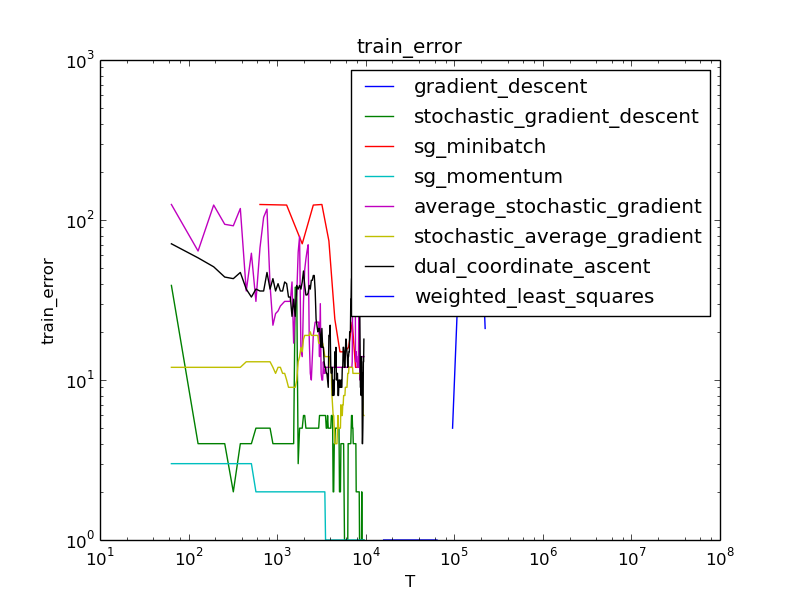
\includegraphics[width = .8\textwidth]{../results/train_error.png}
	\caption{Train error for all methods}
	\label{fig1}
\end{figure}

\begin{figure}[h]
	\centering
	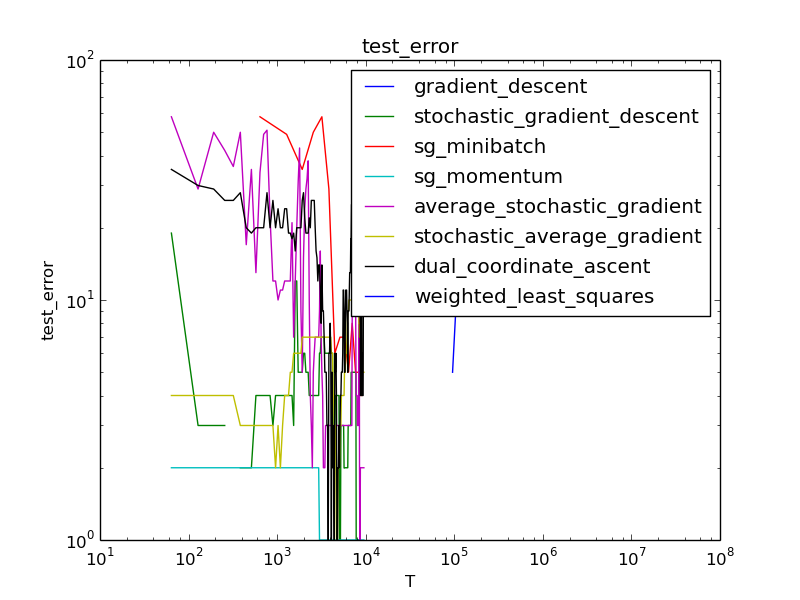
\includegraphics[width = .8\textwidth]{../results/test_error.png}
	\caption{Test error for all methods}
	\label{fig2}
\end{figure}

\FloatBarrier

Unfortunately this representation is quite unorderly, so we also added the course of the test and training error for the individual algorithms in \autoref{fig3} to \autoref{fig}.

\begin{figure}
	\centering
	\begin{subfigure}[b]{0.45\textwidth} 
		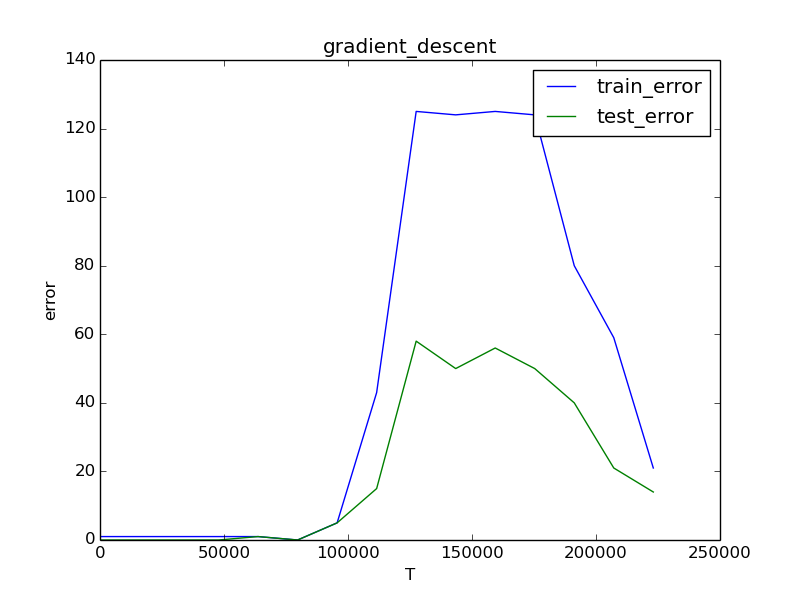
\includegraphics[width=\textwidth]{../results/gradient_descent.png}
		\caption{Results for gradient descent}
		\label{fig3}
	\end{subfigure}
	\begin{subfigure}[b]{0.45\textwidth} 
		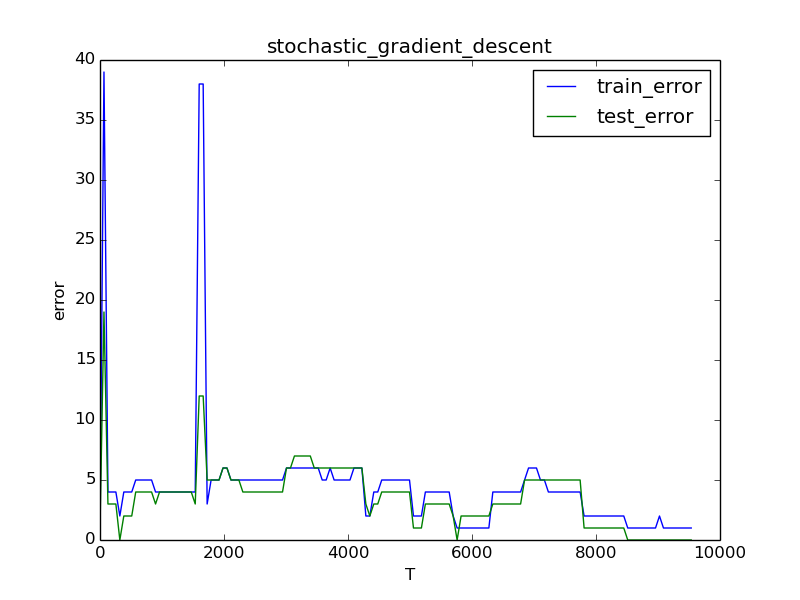
\includegraphics[width=\textwidth]{../results/stochastic_gradient_descent.png}
		\caption{Results for stochastic gradient descent}
		\label{fig4}
	\end{subfigure}
\end{figure}

\begin{figure}
	\centering
	\begin{subfigure}[b]{0.45\textwidth} 
		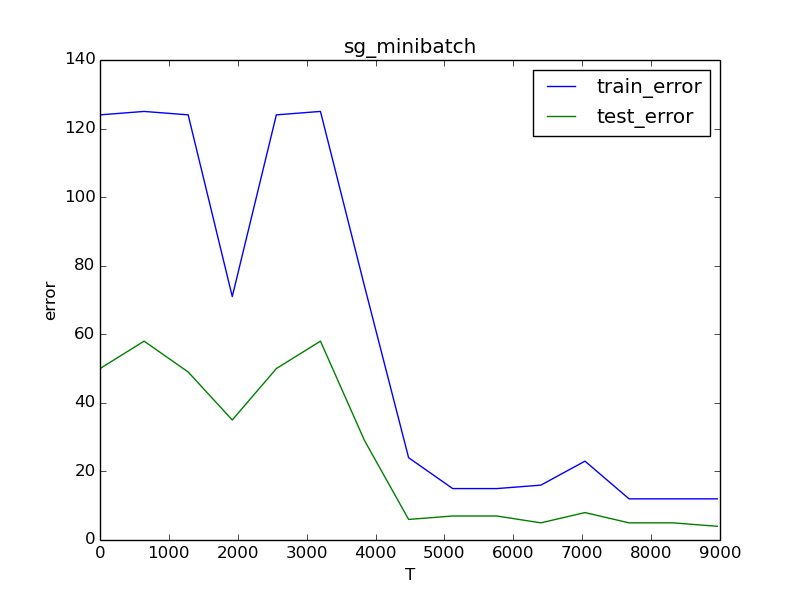
\includegraphics[width=\textwidth]{../results/sg_minibatch.png}
		\caption{Results for SG minibatch}
		\label{fig5}
	\end{subfigure}
	\begin{subfigure}[b]{0.45\textwidth} 
		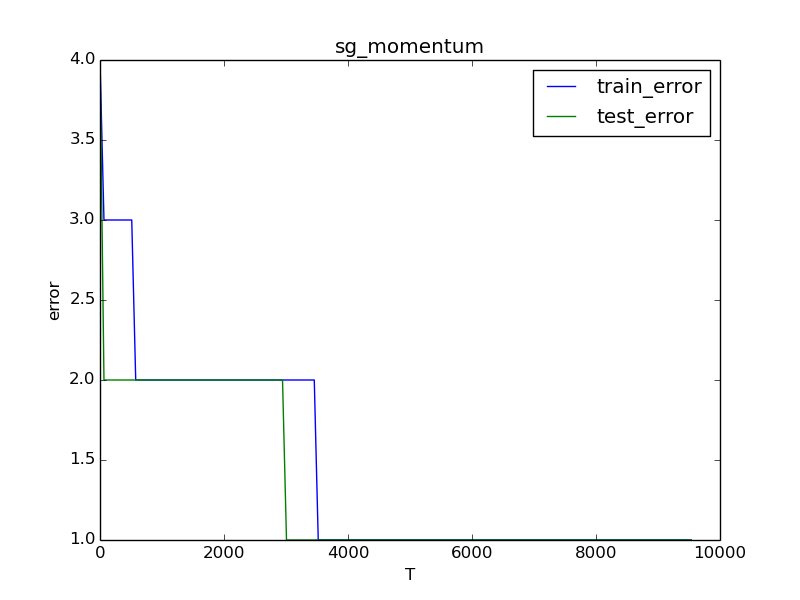
\includegraphics[width=\textwidth]{../results/sg_momentum.png}
		\caption{Results for SG momentm}
		\label{fig6}
	\end{subfigure}
\end{figure}

\begin{figure}
	\centering
	\begin{subfigure}[b]{0.45\textwidth} 
		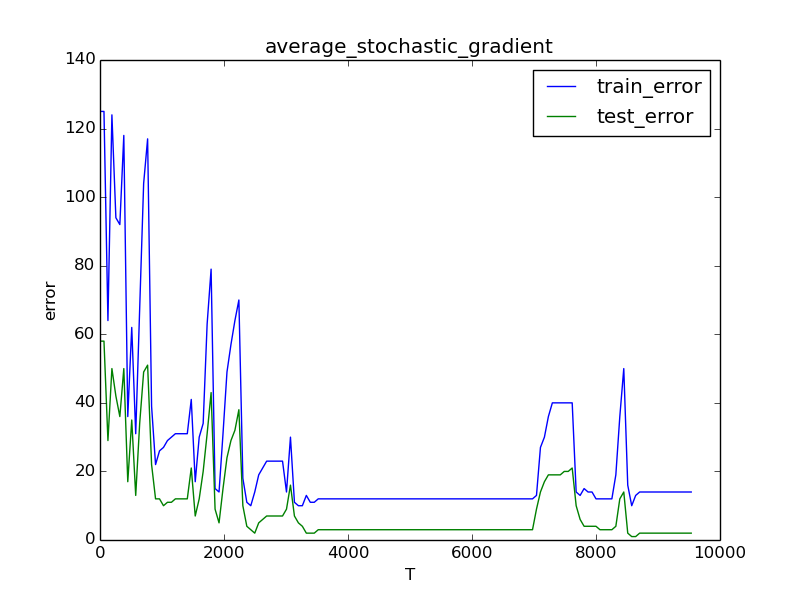
\includegraphics[width=\textwidth]{../results/average_stochastic_gradient.png}
		\caption{Results for average stochastic gradient}
		\label{fig7}
	\end{subfigure}
	\begin{subfigure}[b]{0.45\textwidth} 
		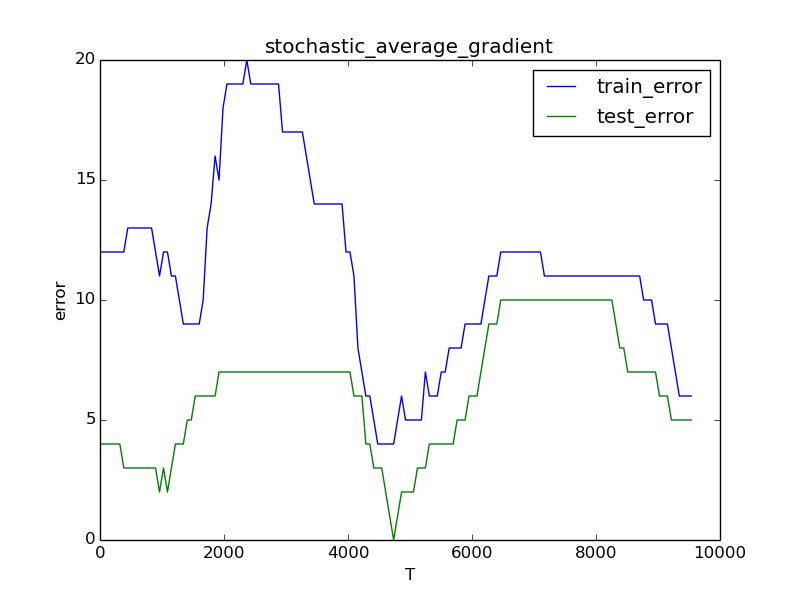
\includegraphics[width=\textwidth]{../results/stochastic_average_gradient.png}
		\caption{Results for stochastic average gradient}
		\label{fig8}
	\end{subfigure}
\end{figure}

\begin{figure}
	\centering
	\begin{subfigure}[b]{0.45\textwidth} 
		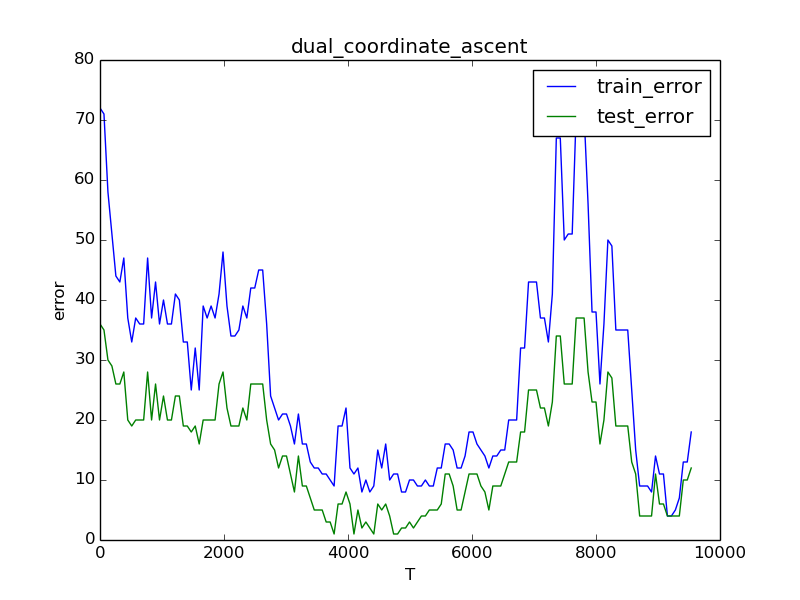
\includegraphics[width=\textwidth]{../results/dual_coordinate_ascent.png}
		\caption{dual coordinate ascent}
		\label{fig9}
	\end{subfigure}
	\begin{subfigure}[b]{0.45\textwidth} 
		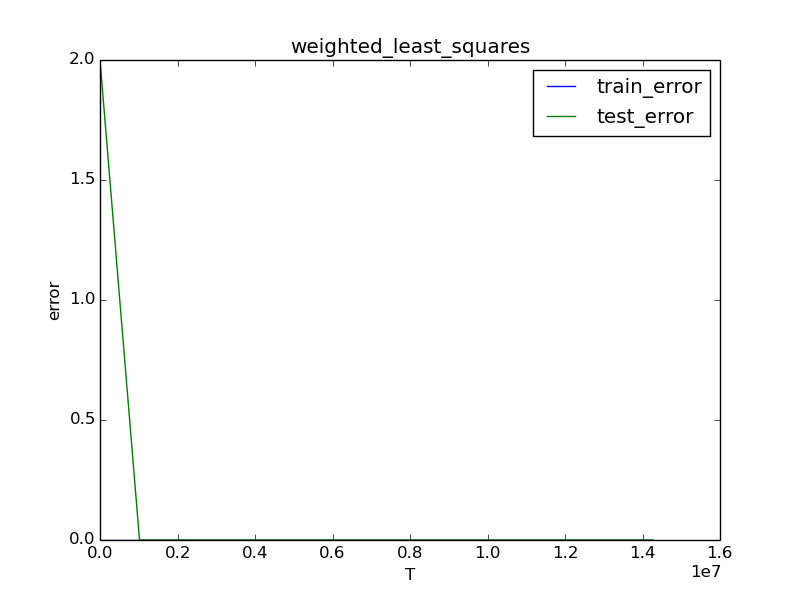
\includegraphics[width=\textwidth]{../results/weighted_least_squares.png}
		\caption{Results for weighted least squares}
		\label{fig10}
	\end{subfigure}
\end{figure}
		
From these plots we can see that most algorithms converge quite orderly. However the gradient descent algorithm, the stochastic average gradient and the dual coordinate ascent show a strange behaviour, in which both test and training error go up again after some time of training.
Unfortunately we did not have further time to look into this behaviour, however for the dual coordinate ascent it might be due to an overflow occuring, which was reported by python.
Overall the SG momemntum algorithm shows the fastest convergence, after T $\approx$ 4000 training and test error have reduced to zero.

\section{Signal Processing}

At last we investigate the relation between SG momentum and SG minibatch / stochastic gradient descent.
From considerations derived from signal processing one expects that these methods show similar convergence behaviour
if one sets $\mu = 1 - e^{- \frac{1}{\eta}}$ for $\eta = 0.6 B$ (minibatch size) , $\eta = 0.6 N$ (trainingset size) respectively.
In the case of SG momentum vs SG minibatch this seems to be approximately the case (see \autoref{fig11}).
However for SG momentum and stochastic gradient descent the momentum algorithm doesnt converge well (see \autoref{fig12}).

\FloatBarrier

\begin{figure}
	\centering
	\begin{subfigure}[b]{0.45\textwidth} 
		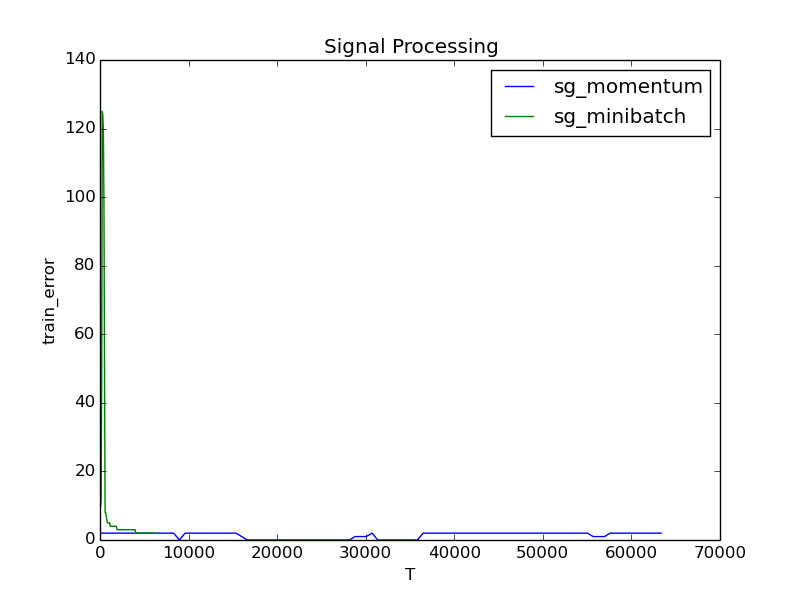
\includegraphics[width=\textwidth]{../results/signal_processing0.png}
		\caption{Comparison of SG momentum and SG minibatch}
		\label{fig11}
	\end{subfigure}
	\begin{subfigure}[b]{0.45\textwidth} 
		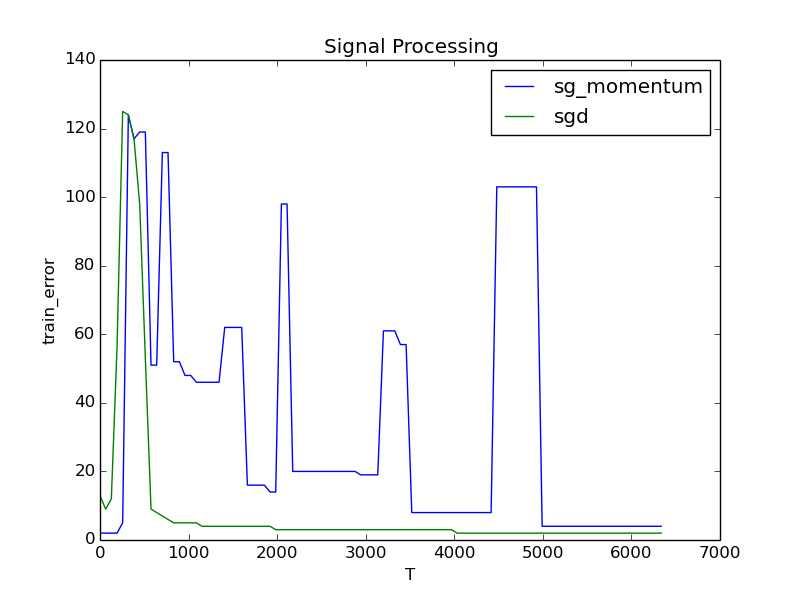
\includegraphics[width=\textwidth]{../results/signal_processing1.png}
		\caption{Comparison of SG momentum and stochastic gradient descent}
		\label{fig12}
	\end{subfigure}
\end{figure}

\end{document}

